\documentclass{X:/Documents/Coding/Latex/myassignment}
\title{Topic C Assignment 4}

\begin{document}

\maketitle

\begin{enumerate}
	\item Use multiple scales to solve
	\[y'' + y + \epsilon(y')^3 = 0\]
	$\epsilon \ll 1$, $y(0)=1$ and $y'(0) = 0$. 

	Let $y(\tau) \sim y_0(t,T)$ where $T=\epsilon t$ is a slow timescale.
	
	
	\begin{align*}
		\dd{}\tau &= \dd{} t + \epsilon\dd{}T\\
		\ddn{}\tau2 &= \ddn{} t2 + 2\epsilon\frac{\partial^2}{\partial t \partial T} + \epsilon^2 \ddn{}T2
	\end{align*}

	Subbing this into the ODE gives:
	\begin{align*}
		\frac{d^2y}{dt^2} + y + \epsilon\left(\odd yt\right)^3 = 0\\
		\ddn{y} t2 + 2\epsilon\frac{\partial^2y}{\partial t \partial T} + \epsilon^2 \ddn{y}T2 + y + \epsilon\left(\dd{y} t + \epsilon\dd{y}T\right)^3 =0 
	\end{align*}
	With initial conditions
	\begin{align*}
		y_0(0,0) &= 1\\
		\dd{y_0(0,0)}{t} = 0 
	\end{align*}
	And
	\begin{align*}
		y_1(0,0) &= 0 \\
		\dd{y_1(0,0)}{t} + y_0(0,0) &= 0
	\end{align*}

	To leading order
	\begin{align*}
		\ddn{y_0} t2  + y_0 =0 \\
		y_0 = R(T)\cos( t + \theta(T))
	\end{align*}
	Boundary conditions:
	\begin{align*}
		y_0(0,0) = 1 \implies R(0) = 1\\
		\dd{y_0(0,0)}{ t} = 0 \implies R(0)(-\sin(\theta(0))) =0 \implies \theta(0) = 0
	\end{align*}
	To obtain the full forms of $R$ and $\theta$, find the second order:
	\begin{align*}
		&\ddn{y_1} t2 + 2\frac{\partial^2y_0}{\partial t \partial T}  + y_1 + \left(\dd{y_0} t\right)^3 =0 \\
		&\ddn{y_1} t2 + 2\left(-R'(T)\sin(t+\theta(T)) -R(T)\cos(t+\theta(T))\theta'(T)  \right) \\& + y_1 + \left(-R(T)\sin(t + \theta(T))\right)^3 =0 \\
	\end{align*}
	\begin{align*}
		\ddn{y_1} t2 + y_1 = 2R'\sin(t + \theta) + 2R\theta' \cos(t + \theta) + R^3 \sin^3(t +\theta)\\
		\ddn{y_1} t2 + y_1 = 2R'\sin(t + \theta) + 2R\theta' \cos(t + \theta) + \frac{R^3}{4} \left(3\sin(t +\theta) - \sin(3(t +\theta))\right)\\
		\ddn{y_1} t2 + y_1 = (2R'+\frac{3}{4}R^3)\sin(t + \theta) + 2R\theta' \cos(t + \theta) - R^3 \left(\sin(3(t +\theta))\right)\\
	\end{align*}
	Hence we require
	\begin{align*}
		(2R'+\frac34R^3) = 0\\
		2R\theta' = 0
	\end{align*}
	For non-trivial solutions this means
	\begin{align*}
		\theta ' =0 \implies \theta = c\\
		2R' + \frac34R^3 = 0 \\
		\frac{R'}{R^3} = - \frac38\\
		-\frac{1}{2R^2} = - \frac38 T + d_*\\
		2R^2 = \frac{1}{\frac38 T -d_*}\\
		R = \pm\frac{1}{\sqrt{\frac34T + d}}
	\end{align*}
	And using the condition from before, $R(0) = 1$
	\begin{align*}
		R = \frac{1}{\sqrt{d}}\\
		\implies d = 1
	\end{align*}
	Hence
	\[\boxed{y_0 = \frac{1}{\sqrt{3T + 1}}\cos(t)}\]

	\begin{figure}[h]
		\centering
		\label{fig:q1}
		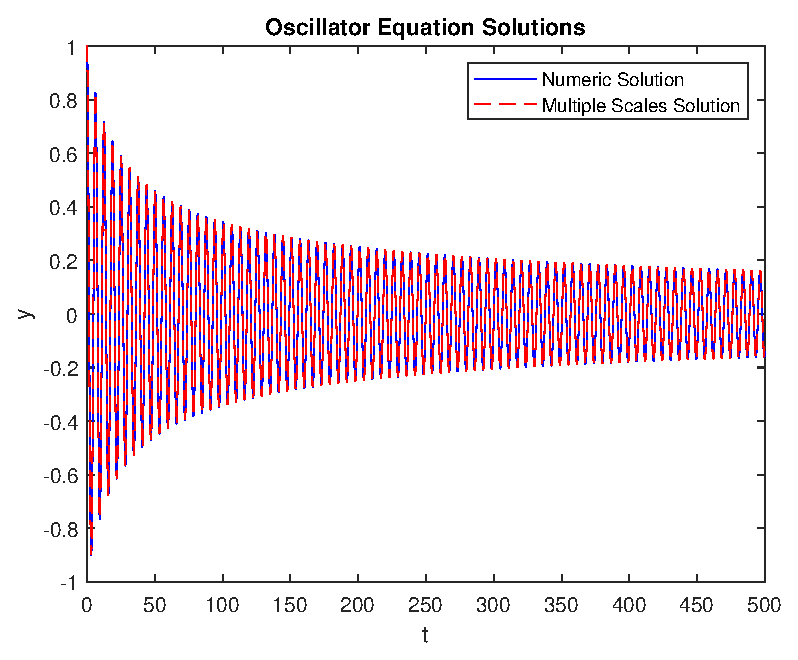
\includegraphics[width=\linewidth]{TopicCA4Q1.eps}
		\caption{Comparison of numerical and multi-scale solutions for $\epsilon = 0.1$}
	\end{figure}


	Figure~\ref{fig:q1} shows the two solutions obtained. Clearly the two overlap very nicely even for $\epsilon=0.1$. 

	%%%%%
	%%Question 2
	%%%%%
	\clearpage
	\item 
	\[\frac{d^2y}{dt^2} + \epsilon(y^2-1)\odd yt + y = 0, \quad y(0) = 1, \ y'(0) = 0, \quad \epsilon\ll 1\]
	\begin{enumerate}
	% \begin{align*}
	% 	\dd{}t &= \dd{}\tau + \epsilon\dd{}T\\
	% 	\ddn{}t2 &= \ddn{}\tau2 + 2\epsilon\frac{\partial^2}{\partial\tau \partial T} + \epsilon^2 \ddn{}T2
	% \end{align*}
		\item %rewrite the ODE as a PDE in t,T,tau Extra slow timescale 
		\[y(t) = y(t,T,\tau)\]
		$T=\epsilon t$ and $\tau = \epsilon^2 t$. 
		This gives the partial derivative expansions:
		\begin{align*}
			\odd{}t &=\dd{}t + \epsilon\dd{}T + \epsilon^2\dd{}\tau\\
			\frac{d^2}{dt^2} &= \dd{}t\left(\dd{}t + \epsilon\dd{}T + \epsilon^2\dd{}\tau\right) + \epsilon\dd{}T\left(\dd{}t + \epsilon\dd{}T + \epsilon^2\dd{}\tau\right) + \epsilon^2 \dd{}\tau\left(\dd{}t + \epsilon\dd{}T + \epsilon^2\dd{}\tau\right)\\
			&= \ddn{}t2 + \epsilon^2 \ddn{}T2 + \epsilon^4\ddn{}\tau2 + 2\epsilon\pdd{}tT + 2 \epsilon^2 \pdd{}t\tau + 2\epsilon^3\pdd{}T\tau
		\end{align*}
		Hence the ODE becomes
		\[\ddn{y}t2 + \epsilon^2 \ddn{y}T2 + \epsilon^4\ddn{y}\tau2 + 2\epsilon\pdd{y}tT + 2 \epsilon^2 \pdd{y}t\tau + 2\epsilon^3\pdd{y}T\tau + \epsilon(y^2-1)\left(\dd{y}t + \epsilon\dd{y}T + \epsilon^2\dd{y}\tau\right) + y = 0\]
		With boundary conditions
		\[y(0,0,0) = 1\]
		\[\dd{y(0,0,0)}t + \epsilon\dd{y(0,0,0)}T + \epsilon^2\dd{y(0,0,0)}\tau = 0\]
		\item %perturbation series, write down the leading order, epsilon, and epsilon^2 problems with boundaries
		First expand the PDE
		\begin{align*}
			&\ddn{y}t2 + \epsilon^2 \ddn{y}T2 + \epsilon^4\ddn{y}\tau2 + 2\epsilon\pdd{y}tT + 2 \epsilon^2 \pdd{y}t\tau + 2\epsilon^3\pdd{y}T\tau \\
			&+ y^2\epsilon\dd{y}t + y^2\epsilon^2\dd{y}T + y^2\epsilon^3\dd{y}\tau- \left(\epsilon\dd{y}t + \epsilon^2\dd{y}T + \epsilon^3\dd{y}\tau\right) + y = 0	
		\end{align*}
		We are only considering up to $\bigo(\epsilon^2)$, so dropping $\epsilon^3$ and higher terms

		\begin{align*}
			&\ddn{y}t2 + \epsilon^2 \ddn{y}T2 + 2\epsilon\pdd{y}tT + 2 \epsilon^2 \pdd{y}t\tau \\
			&+ y^2\epsilon\dd{y}t + y^2\epsilon^2\dd{y}T- \left(\epsilon\dd{y}t + \epsilon^2\dd{y}T \right) + y = 0
		\end{align*}

		Let 
		\[y(t,T,\tau) = y_0(t,T,\tau) + \epsilon y_1(t,T,\tau) + \epsilon^2 y_2(t,T,\tau) + \ldots\]

		\begin{align*}
			&\ddn{y}t2 + \epsilon^2 \ddn{y}T2 + 2\epsilon\pdd{y}tT + 2 \epsilon^2 \pdd{y}t\tau \\
			&+ y^2\epsilon\dd{y}t + y^2\epsilon^2\dd{y}T- \left(\epsilon\dd{y}t + \epsilon^2\dd{y}T \right) + y = 0\\\\
			&\ddn{y_0}t2 + \epsilon\ddn{y_1}t2 + \epsilon^2\ddn{y_2}t2 + \epsilon^2 \ddn{y_0}T2 + 2\epsilon\pdd{y_0}tT + 2\epsilon^2 \pdd{y_1}tT + 2 \epsilon^2 \pdd{y_0}t\tau \\
			&+ y_0^2\epsilon\dd{y_0}t +y_0^2\epsilon^2 \dd{y_1}t +  y_0^2\epsilon^2\dd{y_0}T- \left(\epsilon\dd{y_0}t + \epsilon^2\dd{y_1}t  
			+ \epsilon^2\dd{y_0}T \right) + y_0 + \epsilon y_1 + \epsilon^2 y_2 = 0	
		\end{align*}

		\begin{align*}
			\bigo(1):& \ddn{y_0}t2 + y_0 =0\\
			\bigo(\epsilon):& \ddn{y_1}t2 + 2\pdd{y_0}tT + y_0^2\dd{y_0}t - \dd{y_0}t + y_1 = 0\\
			\bigo(\epsilon^2):& \ddn{y_2}t2 + \ddn{y_0}T2 + 2\pdd{y_1}tT + 2\pdd{y_0}t\tau + y_0^2 \dd{y_1}t + y_0\dd{y_0}T - \dd{y_1}t - \dd{y_0}T + y_2 = 0
		\end{align*}
		With boundary conditions
		\begin{align*}
			\bigo(1):& y_0(0,0,0) = 1, \quad \dd{y_0(0,0,0)}t = 0\\
			\bigo(\epsilon):& y_1(0,0,0) = 0, \quad \dd{y_1(0,0,0)}t + \dd{y_0(0,0,0)}T = 0\\
			\bigo(\epsilon^2):& y_2(0,0,0) = 0, \quad \dd{y_2(0,0,0)}t + \dd{y_1(0,0,0)}T+ \dd{y_0(0,0,0)}\tau = 0\\
		\end{align*}

		\item %find y0 by solving the leading order (and eliminating resonant terms) 
		%can use stuff from lectures
		Leading order equation:
		\[\ddn{y_0}t2 + y_0 = 0\]
		Gives
		\[y_0 = R(T,\tau)\cos(t+\theta(T,\tau))\]
		And using the boundary conditions, require $R(0,0) = 1$ and $\theta(0,0) = 0$

		%Everything below here is matlab

		\item %find y1 (use computer algebra bc it will not be easy to solve)
		To find $y_1$ first sub $y_0$ into the $\bigo(\epsilon)$ equation
		\begin{align*}
			\ddn{y_1}t2 + 2\pdd{y_0}tT + y_0^2\dd{y_0}t - \dd{y_0}t + y_1 = 0\\
			\ddn{y_1}t2 + 2\left(\right) + y_0^2\dd{y_0}t - \dd{y_0}t + y_1 = 0\\
		\end{align*}
		\item %identify the resonant terms in epsilon^2 which contain derivatives of the unknown function of tau in y0. Set one of these to 0 by funding the unknown functions (one is easy to solve, the other look at T to infty)
		\[\ddn{y_2}t2 + \ddn{y_0}T2 + 2\pdd{y_1}tT + 2\pdd{y_0}t\tau + y_0^2 \dd{y_1}t + y_0\dd{y_0}T - \dd{y_1}t - \dd{y_0}T + y_2 = 0\]
		


		\item %compare with numerics and comment
	\end{enumerate}
\end{enumerate}	


\section*{Matlab Code}
\lstinputlisting{AppTopicCA4.m}

\clearpage
\includepdf[pages=1-]{PA_2019_A4.pdf}











\end{document}